% Created 2022-09-12 lun 22:24
% Intended LaTeX compiler: pdflatex
\documentclass[12pt]{article}
\usepackage[utf8]{inputenc}
\usepackage[T1]{fontenc}
\usepackage{graphicx}
\usepackage{grffile}
\usepackage{longtable}
\usepackage{wrapfig}
\usepackage{rotating}
\usepackage[normalem]{ulem}
\usepackage{amsmath}
\usepackage{textcomp}
\usepackage{amssymb}
\usepackage{capt-of}
\usepackage{hyperref}
\usepackage[spanish]{babel}
\usepackage{graphicx,geometry}
\geometry{ a4paper, left=1in, right=1in, top=1in, bottom=1in }
\renewcommand\familydefault{\sfdefault}
\usepackage{sectsty}
\sectionfont{\normalfont\large }
\usepackage{tabularx}
\usepackage{listings}
\lstdefinestyle{mystyle}{
numbers=left,
showspaces=false,
frame=leftline,
showspaces=false,
showstringspaces=false,
showtabs=false,
numberstyle=\tiny,
}
\lstset{
style=mystyle,
literate={á}{{\'a}}1
{é}{{\'e}}1
{í}{{\'{\i}}}1
{ó}{{\'o}}1
{ú}{{\'u}}1
{Á}{{\'A}}1
{É}{{\'E}}1
{Í}{{\'I}}1
{Ó}{{\'O}}1
{Ú}{{\'U}}1
{ü}{{\"u}}1
{Ü}{{\"U}}1
{ñ}{{\~n}}1
{Ñ}{{\~N}}1
{¿}{{?``}}1
{¡}{{!``}}1
}
\makeatletter
\usepackage{fancyhdr}
\pagestyle{fancy}
\usepackage{mdframed}
\BeforeBeginEnvironment{minted}{\begin{mdframed}}
\AfterEndEnvironment{minted}{\end{mdframed}}
\author{Luis Eduardo Galindo Amaya (1274895)}
\date{2022-09-12}
\title{Exploración de los componentes de una interfaz de usuario}
\hypersetup{
 pdfauthor={Luis Eduardo Galindo Amaya (1274895)},
 pdftitle={Exploración de los componentes de una interfaz de usuario},
 pdfkeywords={},
 pdfsubject={},
 pdfcreator={Emacs 26.3 (Org mode 9.1.9)}, 
 pdflang={Spanish}}
\begin{document}


\newcommand{\docente}{Manuel Castañón-Puga}
\newcommand{\asignatura}{Herramientas de Desarrollo de Software (40017)}
\newcommand{\semestre}{2022-2}

\newcommand{\miportada}[1]{
	\begin{titlepage}
		\vspace*{0.75in}
		\begin{flushleft}
			\sffamily
			\large #1       \\
			\Huge 
            \@title         \\
			\hrulefill
			\vspace{0.25in} \\
			\Large \@author \\
			\vspace*{\fill}
            
\includegraphics[width=\textwidth]{../includes/filler.png} \\
			\vspace*{\fill}
			\large
			\begin{tabular}{|l|l|}
              \hline
			  Asignatura & \asignatura \\
			  Docente    & \docente    \\
			  Fecha      & \@date      \\
              \hline
			\end{tabular}
		\end{flushleft}
	\end{titlepage}
}

\fancyhf{}
\lhead{ \asignatura }
\rhead{ \semestre }
\rfoot{Página \thepage}

\setlength\parindent{0pt}   % eliminar el intentado
\setlength{\parskip}{1.2em}
% \maketitle

\thispagestyle{empty}
\begin{center}
	{\large
		UNIVERSIDAD AUTÓNOMA DE BAJA CALIFORNIA \\
		Facultad de Ciencias Químicas e Ingeniería }
	\vspace{0.25in} \\
	Programa de Ingeniero en Software y Tecnologías Emergentes
\end{center}

\section*{Información De La Materia}
\label{sec:orgdb0c26e}
\begin{mdframed}
\begin{description}
\item[{Asignatura}] \asignatura .
\item[{Grupo y Periodo}] 341 (2022-2) .
\item[{Docente}] \docente .
\end{description}
\end{mdframed}

\section*{Información De La Actividad}
\label{sec:orgfd8dc67}
\begin{mdframed}
\begin{description}
\item[{Nombre de la actividad}] Exploración de los componentes de una interfaz de usuario
\item[{Fecha}] 2022-09-12
\item[{Lugar}] Edificio 6E, Salón 204.
\item[{Carácter de la actividad}] Individual.
\item[{Participante(es)}] Luis Eduardo Galindo Amaya (1274895).
\end{description}
\end{mdframed}

\section*{Reporte De Actividades}
\label{sec:org4763368}
\subsection*{Visual Paradigm}
\label{sec:org708a0d8}
Las herramientas son bastante buenas aunque no tiene mucha variedad en tipografías pero una solución bastante solida, quizá le falta una opción colaborativa pero por el resto esta bastante bien.

\begin{center}
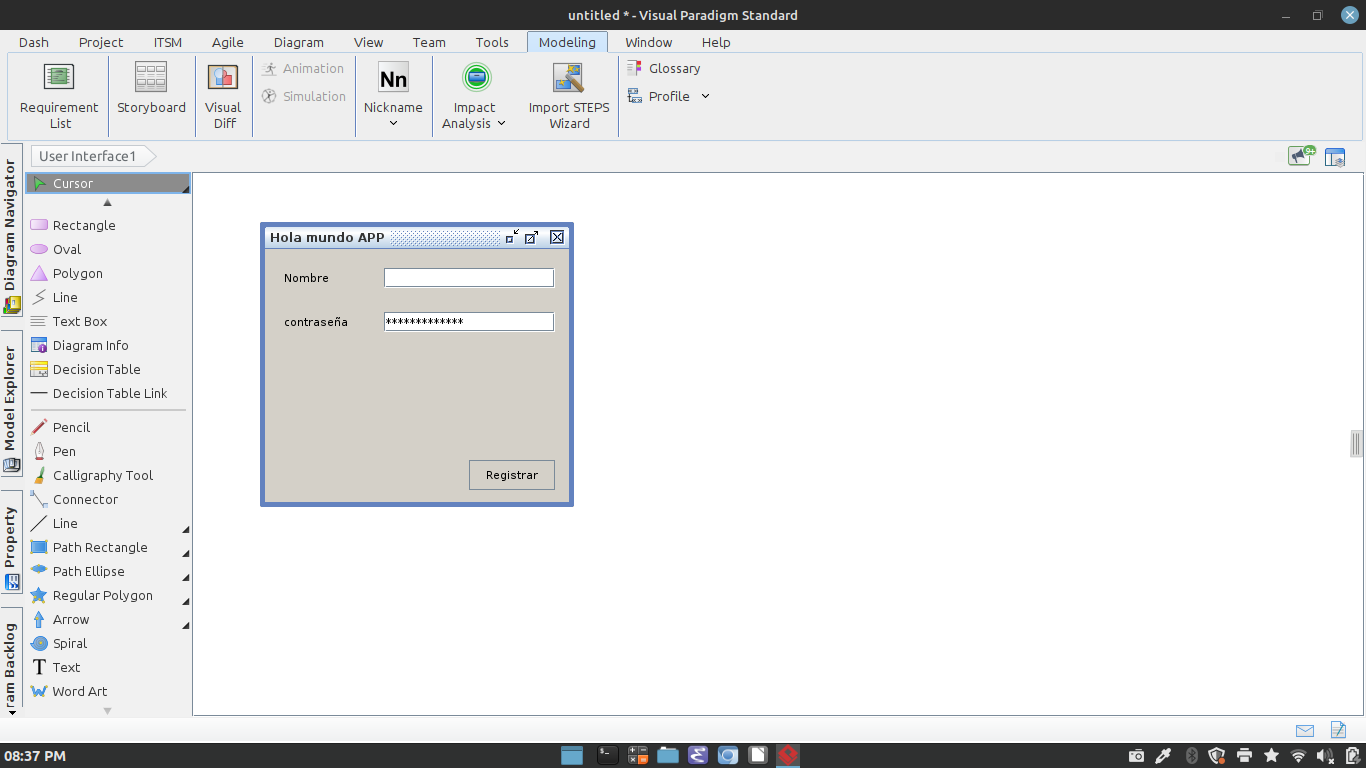
\includegraphics[width=.9\linewidth]{img/VP.png}
\end{center}

\subsection*{mockittapp}
\label{sec:org248910f}
Muy sencilla de usar, quizá en un par de horas de usarla puedes hacer unos diseños muy buenos además que se pueden ajustar todos los parámetros de los labels.

\begin{center}
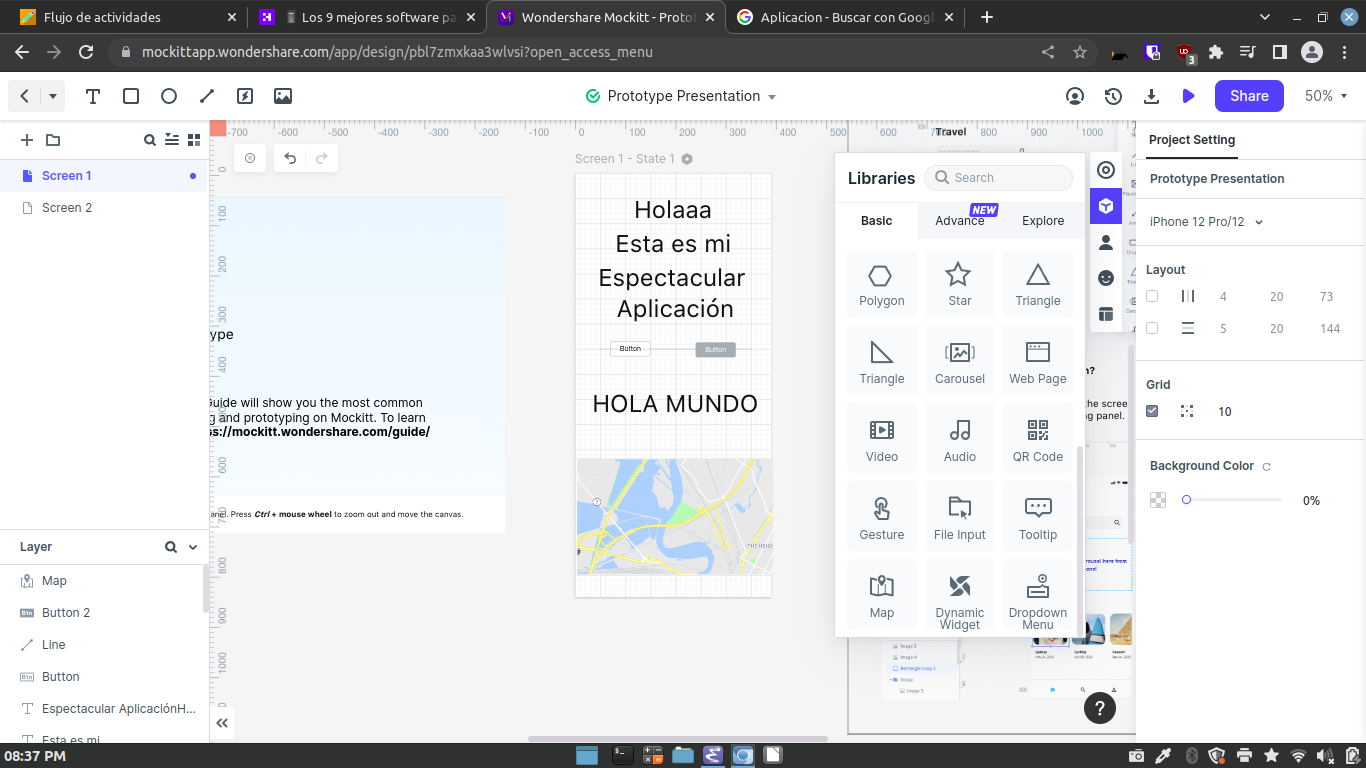
\includegraphics[width=.9\linewidth]{img/mockittapp.png}
\end{center}

\subsection*{gomockingbird}
\label{sec:org8247429}
Una solución mas orientada a las paginas web quizá tiene un layout muy permisivo y no tiene ningún gris para orientarse.

\begin{center}
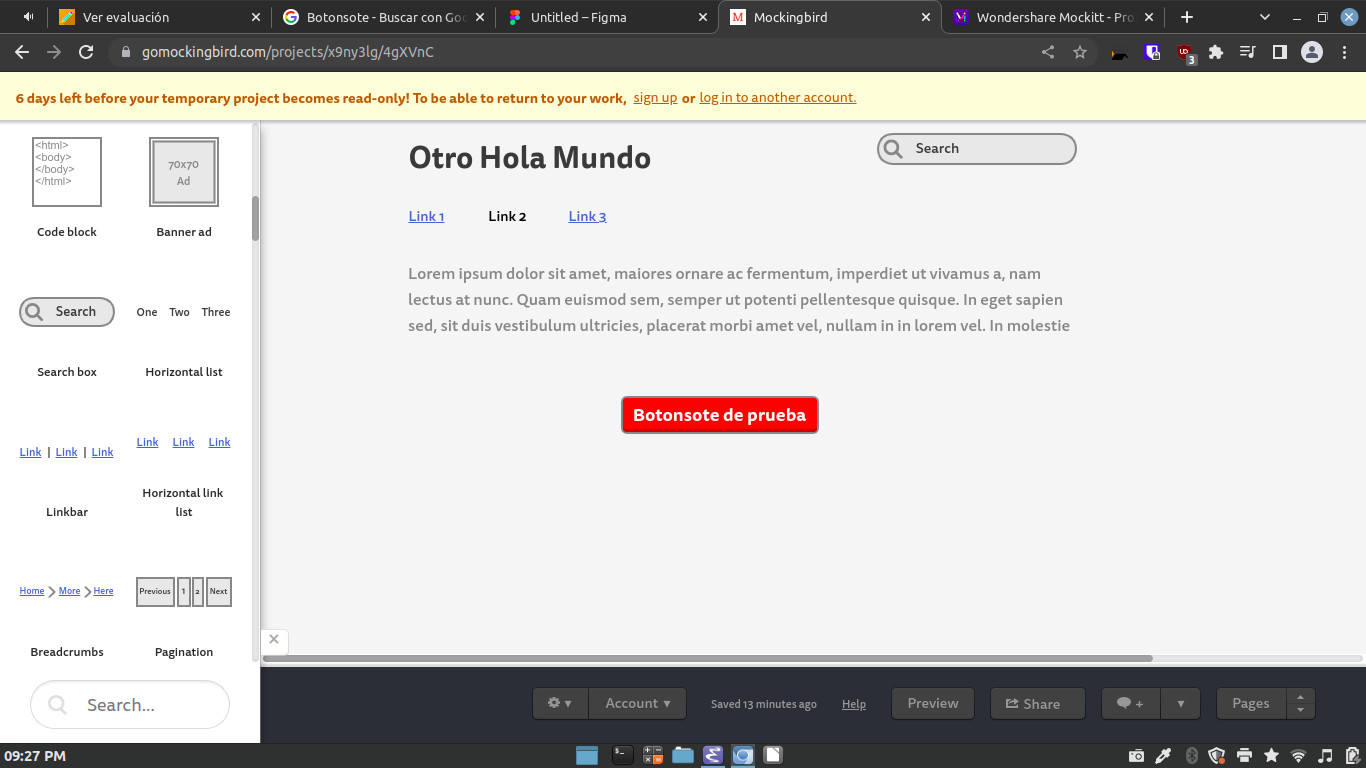
\includegraphics[width=.9\linewidth]{img/gomockingbird.png}
\end{center}

\subsection*{figma}
\label{sec:orgc7d2c3f}
Realmente me tomo bastante rato entender como funciona Figma, me imagino que puede ser una herramienta muy poderosa gracias a sus plugins pero su curva de aprendizaje es un poco mas empinada.

\begin{center}
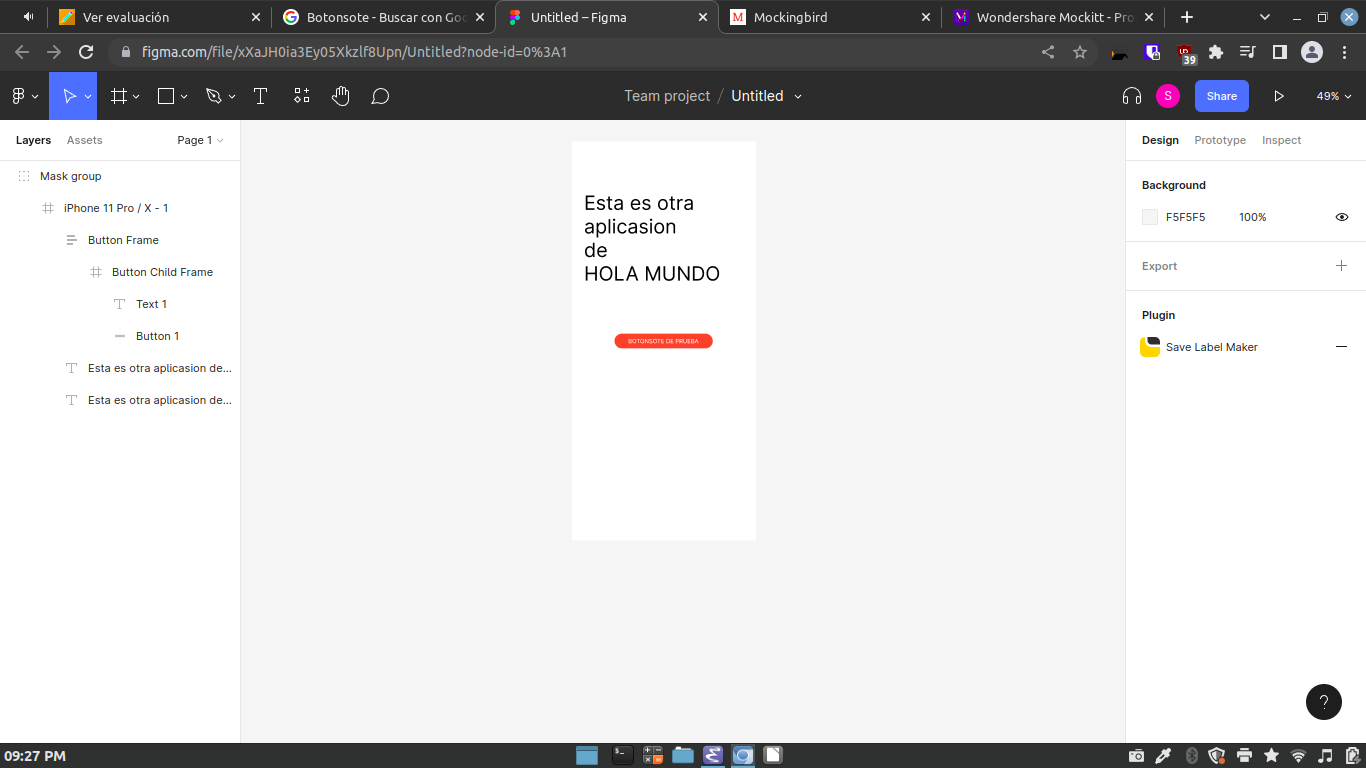
\includegraphics[width=.9\linewidth]{img/figma.png}
\end{center}


\section*{Reflexión}
\label{sec:orgf7d68c1}
\begin{mdframed}
Las interfaces de usuario son indispensables al momento de diseñar un proyecto, que el stakeholder pueda ver como se como sera el proyecto le permite saber si lo que estamos haciendo cumple sus necesidades.
\end{mdframed}

\begin{center}
Doy fe de que toda la información dada es  completa y correcta. \\
\begin{center}

\includegraphics[width=3cm]{../includes/firma.png}
\end{center}
Luis Eduardo Galindo Amaya (1274895)
\end{center}
\end{document}
